\documentclass[12pt,a4paper]{article} 
\usepackage[T1]{fontenc}
\usepackage[francais]{babel}
\usepackage[latin1]{inputenc}
\usepackage{amsmath}
\usepackage{amssymb} %pour des symboles mathematique
\usepackage{graphicx} 
\usepackage{epstopdf} %pour utiliser les .eps
\usepackage{url}
\usepackage{fancyhdr}
\usepackage{fullpage}
\usepackage{array}
\usepackage[table]{xcolor} %pour les couleurs
\usepackage{multicol}
\usepackage[babel=true]{csquotes} %pour les citations

\usepackage{adjustbox} %pour resizer les tableaux

%%%% pour l'insertion de code %%%%%
\usepackage{listings}
\usepackage{color}

\definecolor{dkgreen}{rgb}{0,0.6,0}
\definecolor{gray}{rgb}{0,0,0}
\definecolor{mauve}{rgb}{0,0,0}

\lstset{emph={%  
    float, %
    },emphstyle={\color{gray}\bfseries}%
}%

\lstset{frame=tb,
  language=Matlab,
  aboveskip=3mm,
  belowskip=3mm,
  showstringspaces=false,
  columns=flexible,
  basicstyle={\small\ttfamily},
  numbers=none,
  numberstyle=\tiny\color{gray},
  keywordstyle=\color{black},
  commentstyle=\color{dkgreen},
  stringstyle=\color{black},
  identifierstyle=\color{mauve},
  breaklines=true,
  breakatwhitespace=true
  tabsize=3
}

%%%%%%%%%%%%%%%%%%%%%%

%\pagestyle{myheadings}
%\markright{Tableau blanc interactif}

\title{\LARGE \textbf{TP 1 - Project Abstract and Sensor GUI \\ (with file saving corrected)}\\
	\bigskip
	\bigskip
	\large Techniques d'interaction homme-machine}
\author{Aina Rasolonjatovo Alain Nary Andriambelo \\ Samuel Constantino}
\date{21 mars 2014}

\parindent=0cm
\parskip=6pt

\begin{document}
	\maketitle

%%%%%%%%%%%%%%%%%%%%%%%

\section{Project}

\subsection{Abstract}

Our project will be a game where the player has to decrease her/his stress level to win. A cube (or other object) is placed at the center of the screen and rotates at a speed depending on the player's stress. The more stressed s/he is, the faster the cube spins. More game-like features could also be implemented (for example : different game modes (more challenge-focused) ; a scoring system ; things to disturb the player like terrifying sounds, false acceleration, modification of the scene, etc.) depending on the time we have left.

Our tasks will be : for the Blender part, draw a scene with a cube in the middle (and a background, etc), applying speed for the rotation of the cube, and modifying this speed in real time ; for the sensor part, acquire the GSR data, interpret it and translate it as speed, and finally send it to our Blender game. 

In this project, we will mainly work with the GSR data, however, we might also use the accelerometer data for example as another rotation axis, or to task the player with specific movements, or even to modify the scene directly (move the camera...).

\subsection{Block diagram}

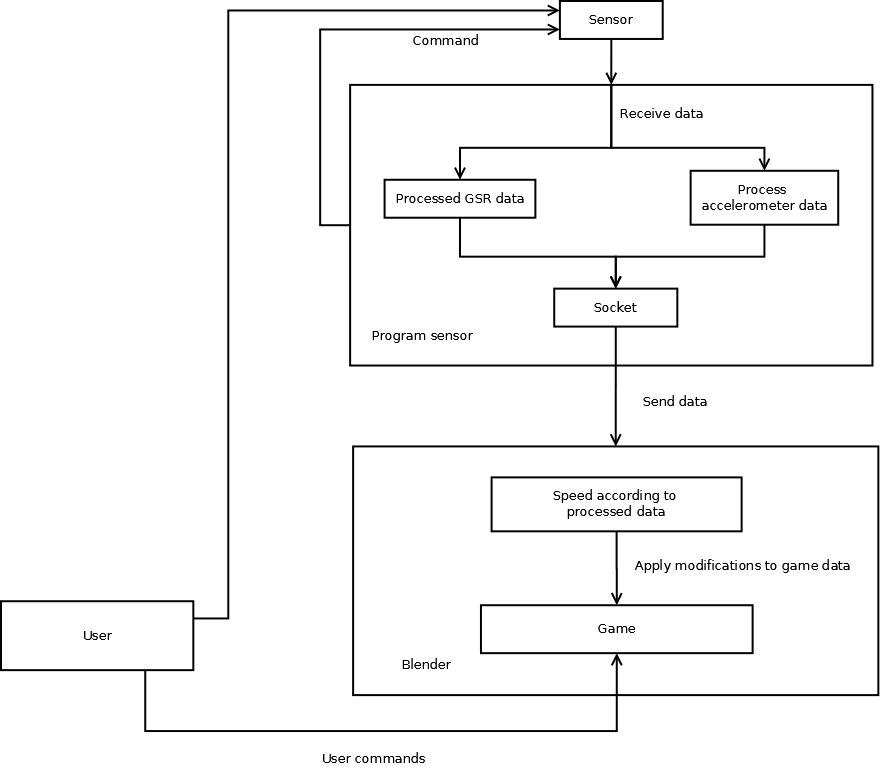
\includegraphics[width=\textwidth,height=\textheight,keepaspectratio]{graph/blockDiagram.png}

\subsection{Use cases}

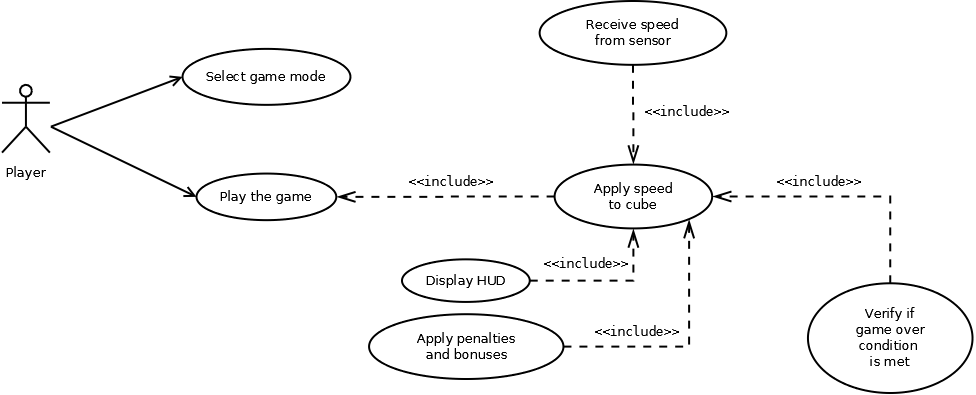
\includegraphics[width=\textwidth,height=\textheight,keepaspectratio]{graph/useCase.png}

When the player launches the game, s/he is prompted with the main menu where s/he can click on two buttons. The first one lets the player decide in which mode to play the game. The second one launches the game. The modes include at least the two following : a 'Relaxation mode' and a 'Challenge mode'. 

In 'Relaxation mode', the player has no real task and can just try to relax as the cube displays her/his stress level in a soothing manner. In 'Challenge mode', the player is tasked with goals (for example, trying to slow the cube to a certain speed, or trying not to variate much from her/his current speed, play in the dark...) for a definite amount of time and wins more time (and score) when a goal is met. The longer s/he plays, the more goals s/he has to complete and the harder these goals are.

In-game, a HUD (head-up display) presents the player with her/his current play-time, current score, on-going goals (in 'Challenge mode'), and the current speed of the rotation. The players only possible action is trying to relax (and complete the goals if any). 

\begin{center}
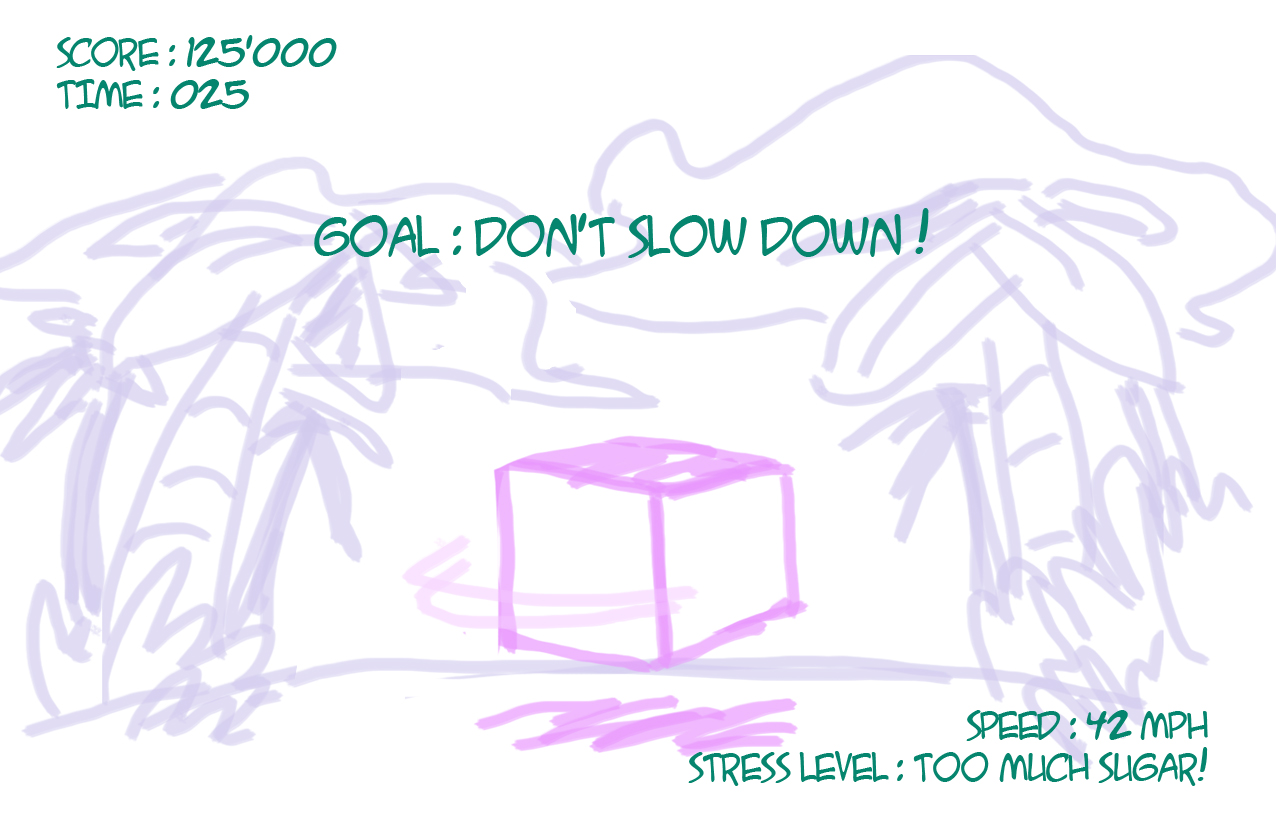
\includegraphics[width=\textwidth,height=\textheight,keepaspectratio]{graph/mockup1.jpg}
\textit{Game screen mockup design}
\end{center}

\clearpage
\section{Interface for accelerometer and electrodermal activity 
 data acquisition}

For this TP, we created a simple interface in Python to visualize the data from the sensor in real-time. The code uses the \texttt{matplotlib} library to make the graphs (http://matplotlib.org/) and the \texttt{pyserial} library to communicate with the sensor (http://pyserial.sourceforge.net/). Both libraries are necessary to run the code. 

\begin{center}
%\includegraphics[width=\textwidth,height=\textheight,keepaspectratio]{graph/figSav01.png}
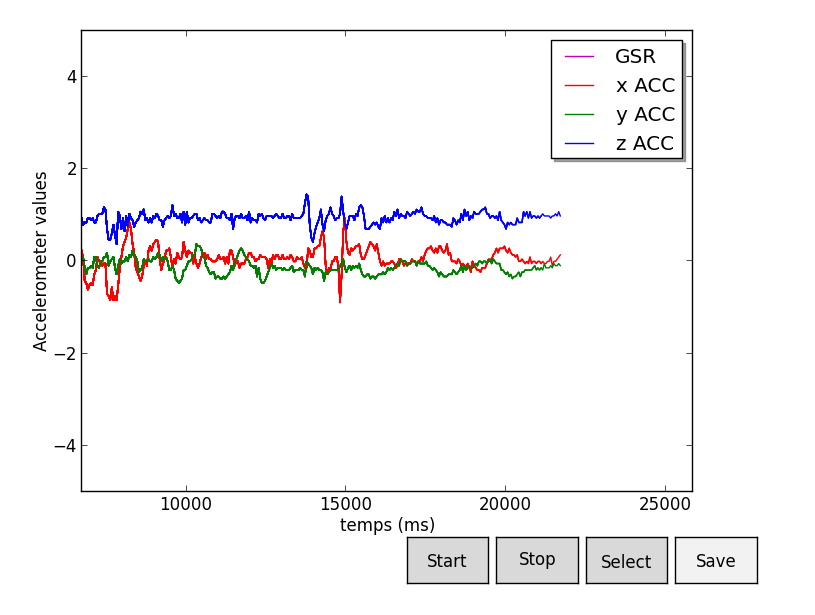
\includegraphics[scale=0.3]{figSav_ACC.png}
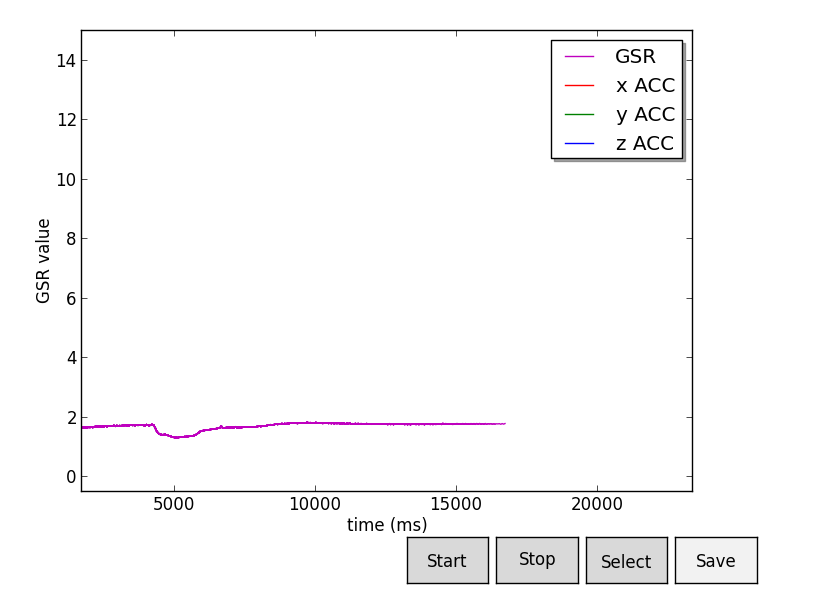
\includegraphics[scale=0.3]{figSav_GSR.png}

\textit{Example our GUI when capturing accelerometer data and GSR data}
\end{center}

The controls for the GUI are the following :
\begin{itemize}
  \item Start : starts capturing the data in real-time
  \item Stop : stops capturing the data
  \item Select : switches between capturing the GSR and accelerometer data
	\item Save : save the captured data (GSR or accelerometer data) in a .txt file
\end{itemize}

\end{document}